%You can leave alone everything before Line 79.
\documentclass{article}
\usepackage{url,amsfonts, amsmath, amssymb, amsthm,color, enumerate}
% Page layout
\setlength{\textheight}{8.75in}
\setlength{\columnsep}{2.0pc}
\setlength{\textwidth}{6.5in}
\setlength{\topmargin}{0in}
\setlength{\headheight}{0.0in}
\setlength{\headsep}{0.0in}
\setlength{\oddsidemargin}{0in}
\setlength{\evensidemargin}{0in}
\setlength{\parindent}{1pc}
\newcommand{\shortbar}{\begin{center}\rule{5ex}{0.1pt}\end{center}}
%\renewcommand{\baselinestretch}{1.1}
% Macros for course info
\newcommand{\courseNumber}{ME 552}
\newcommand{\courseTitle}{Mechatronics}
\newcommand{\semester}{Fall 2012}
\newcommand{\xxx}[1]{\textcolor{red}{#1}}
% Theorem-like structures are numbered within SECTION units
\theoremstyle{plain}
\newtheorem{theorem}{Theorem}[section]
\newtheorem{lemma}[theorem]{Lemma}
\newtheorem{corollary}[theorem]{Corollary}
\newtheorem{proposition}[theorem]{Proposition}
\newtheorem{statement}[theorem]{Statement}
\newtheorem{conjecture}[theorem]{Conjecture}
\newtheorem{fact}{Fact}
%definition style
\theoremstyle{definition}
\newtheorem{definition}[theorem]{Definition}
\newtheorem{example}{Example}
\newtheorem{problem}[theorem]{Problem}
\newtheorem{exercise}{Exercise}
\newtheorem{algorithm}{Algorithm}
%remark style
\theoremstyle{remark}
\newtheorem{remark}[theorem]{Remark}
\newtheorem{reduction}[theorem]{Reduction}
%\newtheorem{question}[theorem]{Question}
\newtheorem{question}{Question}
%\newtheorem{claim}[theorem]{Claim}
%
% Proof-making commands and environments
\newcommand{\beginproof}{\medskip\noindent{\bf Proof.~}}
\newcommand{\beginproofof}[1]{\medskip\noindent{\bf Proof of #1.~}}
\newcommand{\finishproof}{\hspace{0.2ex}\rule{1ex}{1ex}}
\newenvironment{solution}[1]{\medskip\noindent{\bf Problem #1.~}}{\shortbar}

%====header======
\newcommand{\solutions}[4]{
%\renewcommand{\thetheorem}{{#2}.\arabic{theorem}}
\vspace{-2ex}
\begin{center}
{\small  \courseNumber, \courseTitle
\hfill {\Large \bf {#1} }\\
\semester, University of Michigan, Ann Arbor \hfill
{\em Date: #3}}\\
\vspace{-1ex}
\hrulefill\\
\vspace{4ex}
{\LARGE Lab Assignment #2}\\
\vspace{2ex}
\end{center}
\begin{trivlist}
\item \textsc{Team members:\\} {#4}
\end{trivlist}
\noindent
\shortbar
\vspace{3ex}
}
% math macros
\newcommand{\defeq}{\stackrel{\textrm{def}}{=}}
\newcommand{\Prob}{\textrm{Prob}}
%==
\usepackage{graphicx}
\begin{document}
%%%%%%%%%%%%%%%%%%%%%%%%%%%%%%%%%%%%%%%%%%%%%%%%%
%\solutions{Your name}{Problem Set Number}{Date of preparation}{Collaborators}{Prover}{Verifiers}
\solutions{}{1}{\today}{Shiva Ghose, @gshiva\\ John Peterson, @jrpeters\\ Wenjian Bai, @baiwenji}
%%%%%%%%%%%%%%%%%%%%%%%%%%%%%%%%%%%%%%%%%%%%%%%%%
%\renewcommand{\theproblem}{\arabic{problem}} 
%%%%%%%%%%%%%%%%%%%%%%%%%%%%%%%%%%%%%%%%%%%%%%%%%
%
% Begin the solution for each problem by
% \begin{solution}{Problem Number} and ends it with \end{solution}
%
% the solution for Problem 

\section*{Question 1}
\subsection*{a}
The circuit diagram can be seen in figure \ref{q1_a}.
\begin{figure}[h]
\begin{center}
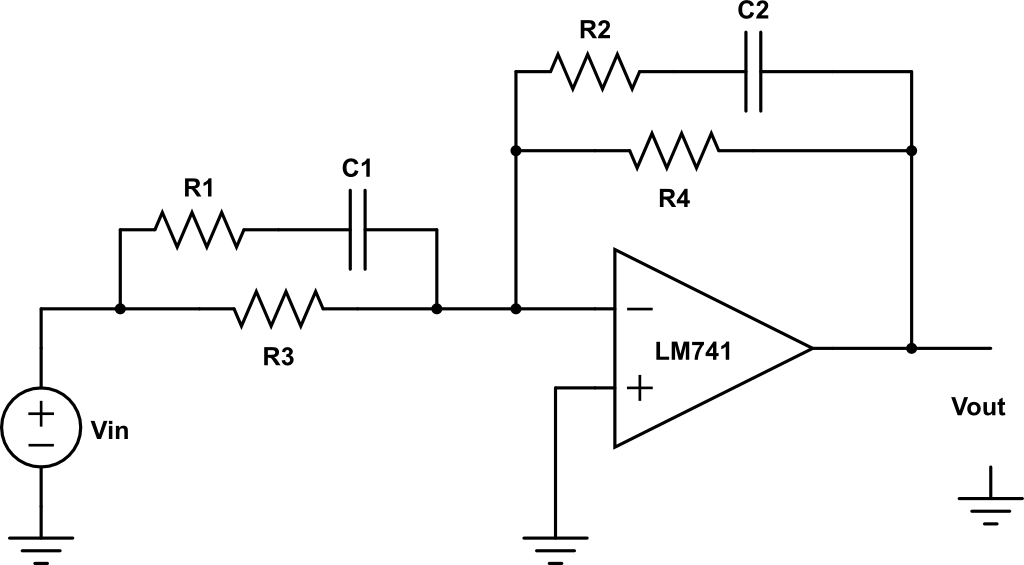
\includegraphics[width=10cm]{q1_circuitDiagram.png}
\end{center}
\caption{A lead-lag compensator circuit diagram for question 1.}
\label{q1_a}
\end{figure}

\subsection*{b}
If we consider the impedance of the group $R_1$, $C_1$ and $R_3$ as $Z_1$ and the impedance of the group  $R_2$, $C_2$ and $R_4$ as $Z_2$, we can get the circuit diagram seen in figure \ref{q1_b}.This circuit essentially operates as an inverting amplifier and hence the relationship between the output and input is given as:
\begin{figure}[h]
\begin{center}
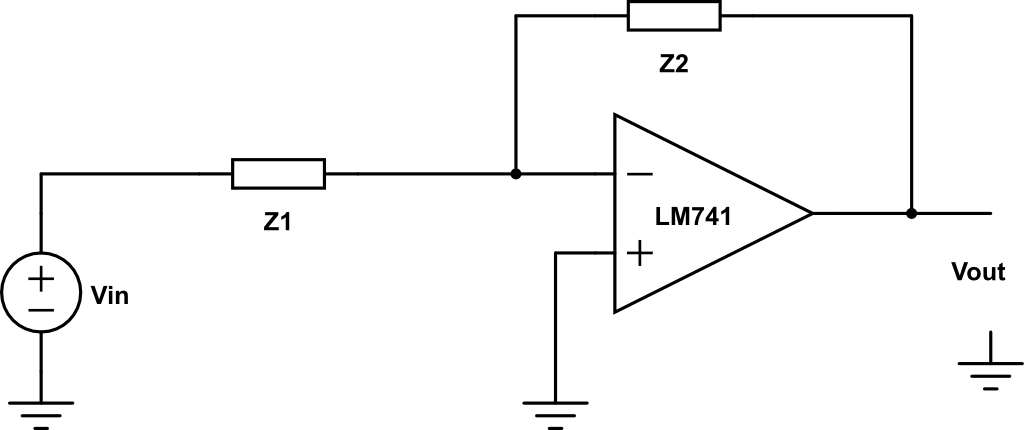
\includegraphics[width=10cm]{revised-lead-lag-simplified.png}
\end{center}
\caption{Simplified lead-lag compensator circuit diagram.}
\label{q1_b}
\end{figure}
 

$$\frac{V_{out}(s)}{V_{in}(s)} = - \frac{Z_2}{Z_1}$$
Where:
$$Z_1 = \frac{R_3 * (R_1 + (1/sC_1))}{R_3 + (R_1 + (1/sC_1))} = \frac{R_3(sR_1C_1 +1)}{s(R_1C_1 + R_3C_1) + 1} \ \text{, and}$$
$$Z_2 = \frac{R_4 * (R_2 + (1/sC_2))}{R_4 + (R_2 + (1/sC_2))} = \frac{R_4(sR_2C_2 +1)}{s(R_2C_2 + R_4C_2) + 1}$$
Thus the gain of the system can now be re-written as:
$$\frac{V_{out}(s)}{V_{in}(s)} = -  \frac{R_4(sR_2C_2 +1)}{(s(R_2C_2 + R_4C_2) + 1)}\frac{(s(R_1C_1 + R_3C_1) + 1)}{R_3(sR_1C_1 +1)} $$
$$=  -  \frac{R_4}{R_3}\frac{(sR_2C_2 +1)}{(s(R_2C_2 + R_4C_2) + 1)}\frac{(s(R_1C_1 + R_3C_1) + 1)}{(sR_1C_1 +1)} $$

We see that the op-amp operates as an inverting amplifier. In order to match the required transfer function, we need to account for the additional $-\frac{R_4}{R_3}$ gain, which we can do by passing the output of the circuit through another inverting amplifier which has a gain of $-\frac{R_3}{R_4}$\footnote{For practical purposes this second op-amp is implemented in LabView as a negative gain.}. Comparing our final transfer function with what is asked in the question, we get:

$$\Big( -  \frac{R_4}{R_3} \times -\frac{R_3}{R_4} \Big)\frac{(sR_2C_2 +1)}{(s(R_2C_2 + R_4C_2) + 1)}\frac{(s(R_1C_1 + R_3C_1) + 1)}{(sR_1C_1 +1)}  = \frac{(1+0.1s)(1 + 5s)}{(1+0.01s)(1 + 10s)}$$

Comparing the LHS and the RHS, we see:
$$R_1C_1 = 0.01$$
$$R_2C_2 = 5$$
$$R_1C_1 + R_3C_1 = 0.01 + R_3C_1 = 0.1$$
$$\implies R_3C_1 = 0.09$$
$$R_2C_2 + R_4C_2 = 5 + R_4C_2 = 10$$
$$\implies R_4C_2 = 5$$
$$\therefore R_4 = R_2$$

\subsection*{c}
While building this circuit, we made the following assumptions:
\begin{itemize}
\item The op-amps we use are ideal, i.e. the input impedance is infinite and the output impedance is negligible. This implies that the op-amp does not load it's input circuit and loading effects are not seen on the op-amps output terminal.

\item The voltage at the inverting terminal is equal to the voltage at the non-inverting terminal.

\item The open loop op-amp gain is infinite.

\item The op-amp will operate in an ideal manner when the output is not saturated above or below its supply limits.

\item We assumed that the performance of the system is not overly sensitive to variations in resistance and we assumed the values of that the resistors were accurate and that capacitors had negligible internal resistance.

\end{itemize}

\subsection*{d}
We can determine the ratings of the components by arbitrarily setting $C_1$ and $C_2$. We set the capacitances because the values available to us is limited whereas we have significantly more flexibility with choosing resistances. By fixing $C_1$ and $C_2$ we find:
$$R_1 = \frac{0.01}{C_1}$$
$$R_2 = \frac{5}{C_2}$$
$$R_3 = \frac{0.09}{C_1} \ \text{,  and}$$
$$R_4 = R_2$$

We additionally see that the gain of the inverting op-amp lead-lag circuit is proportional to $ \frac{R_4}{R_3}$. We  want to limit this so that the output does not get saturated while trying to amplify the signal by a large amount. As we need to use an input amplitude of up to 2V in part (\emph{i}), for a input supply of +/- 15V, we would like to limit the op-amp output to +/- 10V. Hence we want the gain,$ \frac{R_4}{R_3}, \approx 5$. 

$$\frac{R_4}{R_3} \approx 5 \implies \frac{(5/C_2)}{(0.09/C_1)} \approx 5$$
$$\therefore \frac{C_1}{C_2} = 0.09$$

For this circuit we chose $C_1 = 2.2 \mu F$, hence ratings of the other components became:\\
\begin{table}[hbt]
\begin{center}
    \begin{tabular}{|c|c|c|}
        \hline
        \textbf{Component Name} & \textbf{Component Type} & \textbf{Component Specification} \\ \hline
       $ LM 741$                     & \text{Signal Op-amp}         & $ \ V+ = +15V, V- = -15V     $             \\	
       $ C_1$                     & \text{Electrolytic Capacitor}         & $ \ 2.2 \mu F     $             \\ 
       $ C_2 $                   & \text{Electrolytic Capacitor}         & $ \ 22 \mu F     $               \\ 
       $ R_1  $                  & \text{Resistor}         & $ \ 454 \Omega            $        \\ 
       $ R_2 $                    & \text{Resistor}         & $ \ 227 K\Omega        $            \\        
       $ R_3 $                   & \text{Resistor}         & $\ 40.9 K\Omega   $                 \\ 
       $ R_4$                     & \text{Resistor}         &$ \ 227 K\Omega$                    \\
        \hline
    \end{tabular}

\caption{Capacitances and Resistances chosen to construct the lead-lag controller}
\label{q1_td}
\end{center}
\end{table}

While choosing the components we ensured that the wattage rating of the components were at least equal to or exceeded the power supply of the circuit. As little or no current passes through the circuit\footnote{The system doesn't draw much power and the output of the system is connected to a measuring device which also theoretically draws no current.}, we used $V^2/ R$ to determine the power rating. In every case, the minimum power rating of the component exceeded the circuit power ratings.


\subsection*{e} We constructed the circuit as described above and collected experimental data as follows.

\subsection*{f}
The theoretical bode plot of the desired system and the actual bode plot obtained are shown in figure \ref{q1_ff}.
\begin{figure}[hbt]
\begin{center}
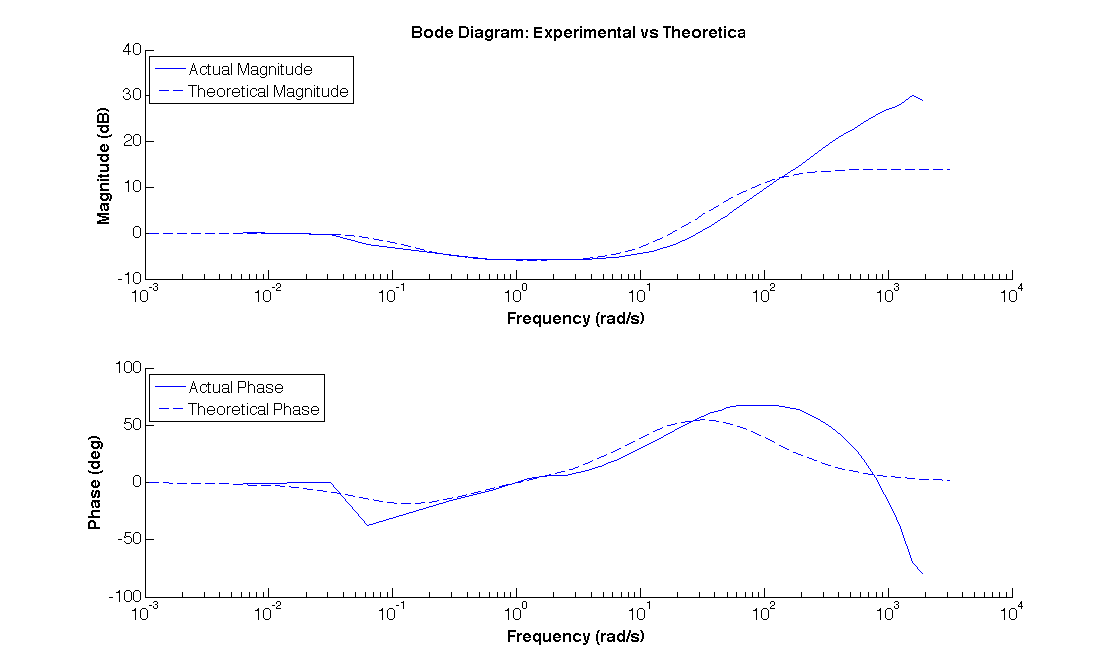
\includegraphics[width = 17cm]{bodeplot.png}
\caption{Bode Plot of Theoretical System and Actual System}
\label{q1_ff}
\end{center}
\end{figure}

\subsection*{g}
Our actual results illustrate the same trends as the theoretical system and have similar gains and phases for the most part, but the actual gain and phase diverge at high frequencies.  The divergence in phase seems to be a symptom of aliasing caused by the limited sampling rate of our DAQ.  Theoretically, sampling at 1000 Hz should allow us to reconstruct the frequency component of the response generated by the system up to 500 Hz but there is no guarantee that the magnitude will be faithfully reconstructed.  At frequencies above 150 Hz we saw that the phase estimate would no longer be reliable and would often jump from large positive to large negative values .  More often than not, the system would illustrate the phase lag illustrated in figure \ref{q1_ff}.  We suspect that the gain estimate deviated for similar reasons. Additionally another cause of discrepancies is the fact that we used physical components instead of theoretical components. This means that the ratings of the components are not exact and in the case of the op-amp, not all the input power is available to the output - this can cause differences.

\subsection*{h}
Table \ref{q1_th} shows the maximum and minimum phase angles present in the bode plot of the actual and theoretical systems.  Note that for the actual system we have omitted the leading portion of the phase diagram above 100 $\frac{rads}{s}$ because we believe it to be an artifact of aliasing.  
\begin{table}[hbt]
\begin{center}
	\begin{tabular}{|c|c|c|}
		\hline
		 & \textbf{Theoretical System} & \textbf{Actual System}  \\ \hline
		Minimum Phase Angle (degrees) & -18.76 &  -37.93\\
		Minimum Phase Frequency (rads/s) & 0.136 & 0.06283\\
		Maximum Phase Angle (degrees) & 54.72 & 67.46 \\ 
		Maximum Phase Frequency (rads/s) & 31.83 & 125.7\\ \hline
	\end{tabular}
\caption{Maximum and Minimum Phase Angles and Frequencies for Theoretical and Actual System}
\label{q1_th}
\end{center}
\end{table}

We notice for the this system when we see a phase lead, it is accompanied by a decrease in the magnitude and we also see that the phase lag at higher frequencies is accompanied by an increase in the magnitude. 

\subsection*{i}

Table \ref{q1_it} shows the output phase and gains obtained when varying the input amplitude from 0.5 V to 2 V at 1Hz and 2Hz input sine waves.  Theoretically we would expect the output phase and amplitude ratio to remain constant at a given frequency for any input amplitude.  The magnitude of the bode plot gives the ratio of the output to input at a particular frequency while the phase portion gives the phase at that frequency and both are independent of the input amplitude. We would of course expect expect the phase and amplitude ratios to vary according to the bode plot across different frequencies.  \\

Experimentally this seems to be the case for a 1Hz input, but it is not the case for the 100 Hz input.  For a 1Hz input frequency the input amplitudes chosen avoid saturating the system, while the 100Hz signal saturates the system such that output can not increase with increasing input voltage. As our system inherently also has an additional gain of 5.556\footnote{$\frac{R_4}{R_3}$ = 5.556}, and due to the fact that we are using non-ideal op-amps that cannot output the entire input-power range, we see that the system saturates while trying to output more than 10.3 Volts.


\begin{table}[hbt]
\begin{center}
    \begin{tabular}{|c|c|c|c|}
        \hline
        Input Frequency (Hz) & Input Amplitude (V) & Output Phase (degrees) & Output Gain \\ \hline
        1                    & 0.5             & 21.0959                & 0.548067               \\ 
        1                    & 1               & 19.8599                & 0.548165               \\ 
        1                    & 2               & 21.1367                & 0.549704               \\ 
        100                  & 0.5             & -24.2329               & 4.83643                \\ 
        100                  & 1               & -23.8303               & 2.61935                \\ 
        100                  & 2               & -24.7609               & 1.23915                \\
        \hline
    \end{tabular}
\end{center}
\caption{Amplitude dependence of system response at two different frequencies}
\label{q1_it}
\end{table}

\subsection*{j}

We generated the Bode Diagram by using a pair of Tone Measurement blocks to extract the amplitude and phase of the input and output signals.  We then took the difference of these phases to compute the phase difference and divided the output amplitude by the input amplitude to compute the system gain.  We selected a range of frequencies, running the system at each frequency and then making note of the resulting phase and amplitude ratio by hand and then plotted these results against the theoretical results in MATLAB.

\begin{figure}[h]
\begin{center}
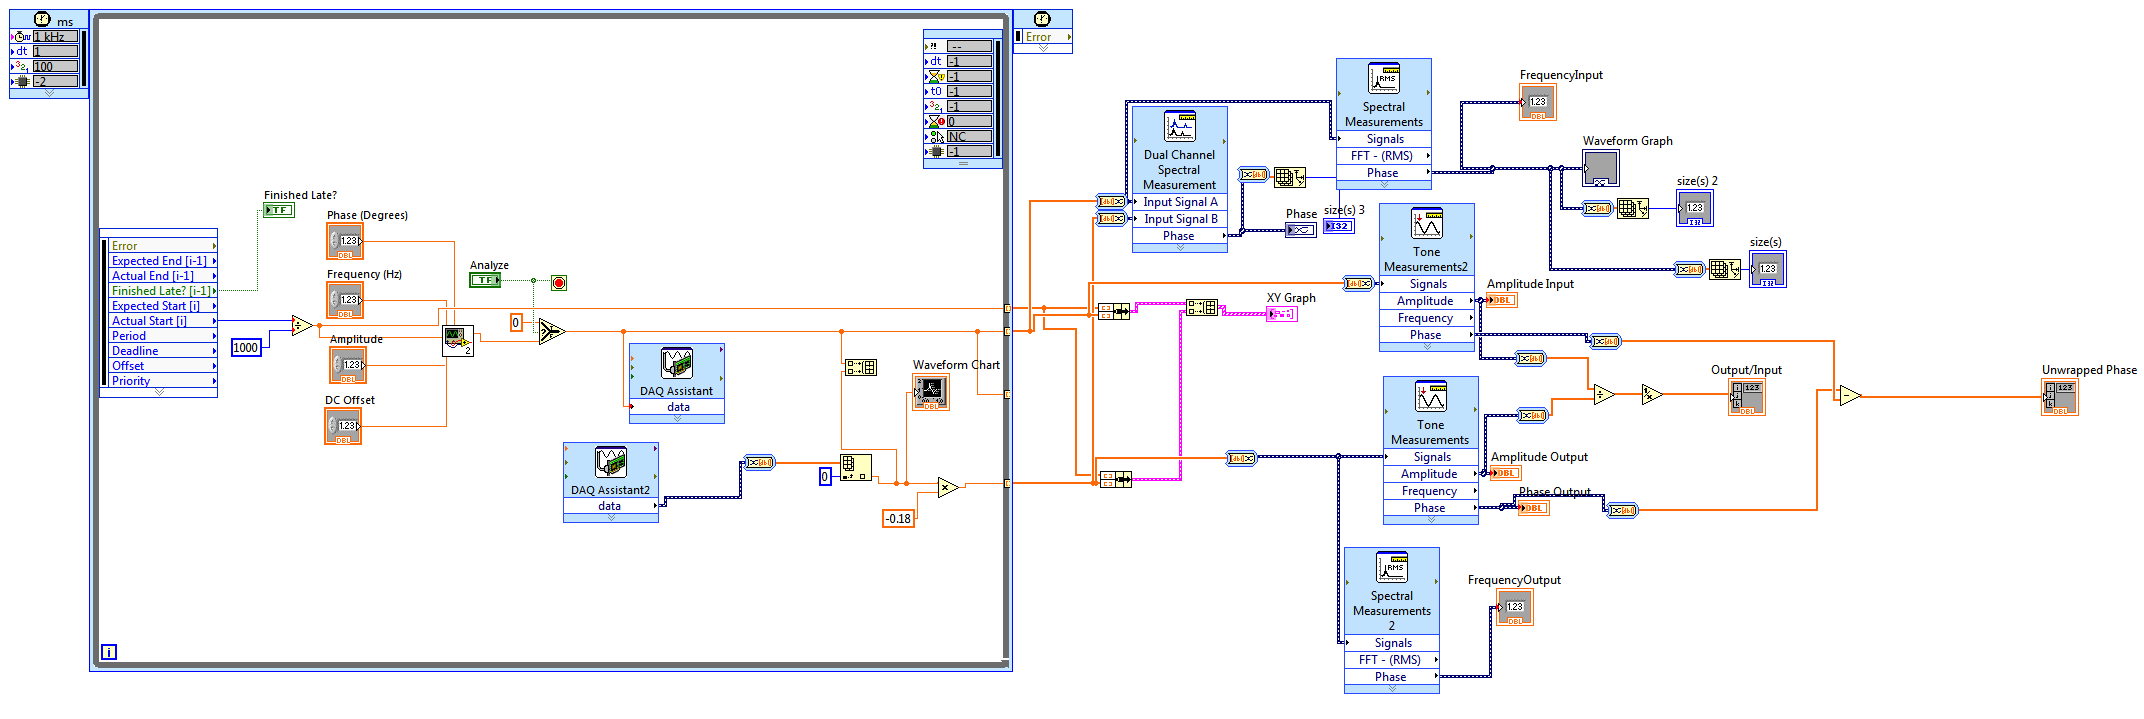
\includegraphics[width = 17cm]{blockDiagram.png}
\caption{LabView Block Diagram for Extracting Phase and Gain}
\label{q1_j1}
\end{center}
\end{figure}

\begin{figure}[h]
\begin{center}
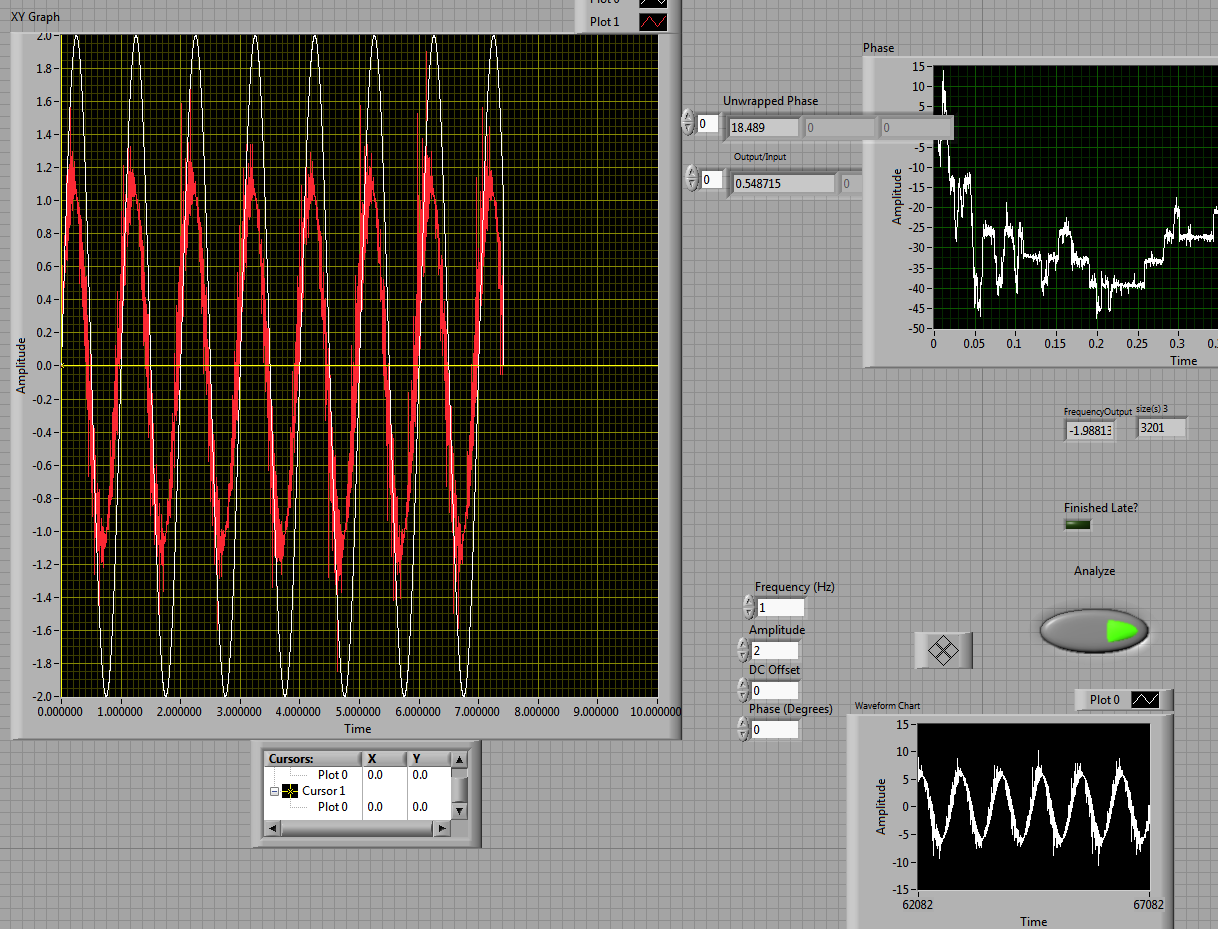
\includegraphics[width = 10cm]{frontPannel.png}
\caption{LabView Front Panel for extracting Phase and Gain}
\label{q1_j2}
\end{center}
\end{figure}

\section*{Question 2}

\subsection*{a}
The circuit diagram is shown in figure \ref{q2_a}.
\begin{figure}[h]
\begin{center}
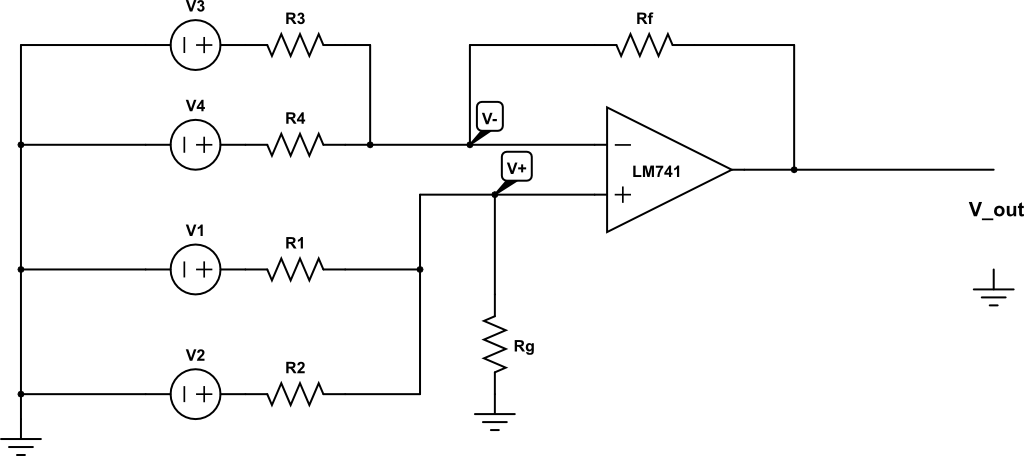
\includegraphics[width=10cm]{q2_circuitDiagram.png}
\end{center}
\caption{The required circuit diagram for question 2.}
\label{q2_a}
\end{figure}


\subsection*{b}
Circuit analysis:\\

At the non-inverting terminal, we effectively have a circuit represented by figure \ref{q2_b1}. We can use Kirchoff's voltage law along with the superposition theorem, we see:
\begin{figure}[h]
\begin{center}
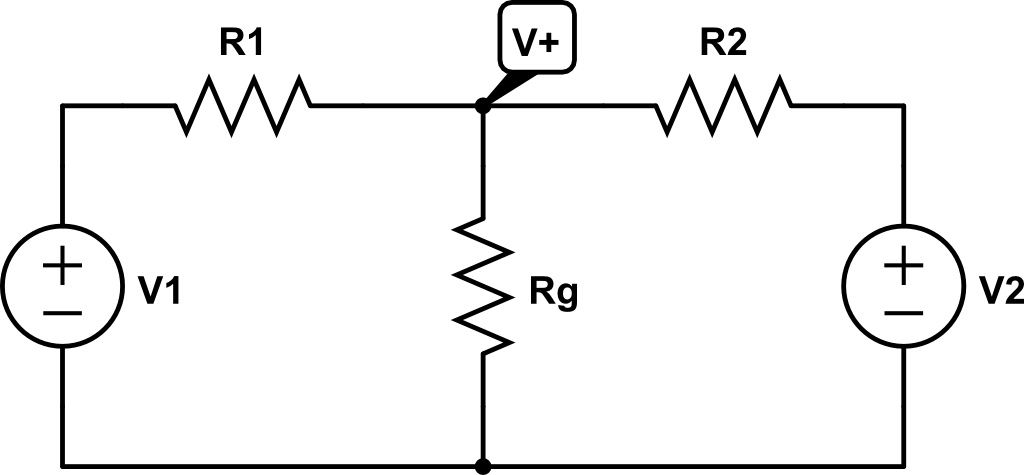
\includegraphics[width=6cm]{lab1_q2_kvl1.png}
\end{center}
\caption{Equivalent circuit at the non-inverting terminal}
\label{q2_b1}
\end{figure}

$$\text{Voltage at $V^+$ due to $V_1$, $V^+_1$, is given by:}$$
$$V^+_1 = \frac{\frac{R_2 R_g}{R_2+R_g}}{R_1 + \frac{R_2 R_g}{R_2+R_g}}\ V_1$$
$$\therefore V^+_1 = \Big(\frac{1}{\frac{R_1}{R_g} + \frac{R_1}{R_2} + 1}\Big) \ V_1$$

$$\text{Similarly, voltage at $V^+$ due to $V_2$, $V^+_2$, is given by:}$$
$$V^+_2 = \frac{\frac{R_1 R_g}{R_1+R_g}}{R_2 + \frac{R_1 R_g}{R_1+R_g}}\ V_2$$
$$\therefore  V^+_2 = \frac{1}{\frac{R_2}{R_g} + \frac{R_2}{R_1} + 1} \ V_2$$

$$\text{Using the superposition theorem to recombine the values, we find that $V+$ is given by:}$$
$$V^+ = V^+_1 + V^+_2 $$
$$V^+ = \frac{1}{\frac{R_1}{R_g} + \frac{R_1}{R_2} + 1} \ V_1 + \frac{1}{\frac{R_2}{R_g} + \frac{R_2}{R_1} + 1} \ V_2 $$

We can now move on to the inverting terminal of the op-amp. The corresponding equivalent circuit is shown in figure \ref{q2_b2}.  Analyzing this circuit, we see that:
\begin{figure}[h]
\begin{center}
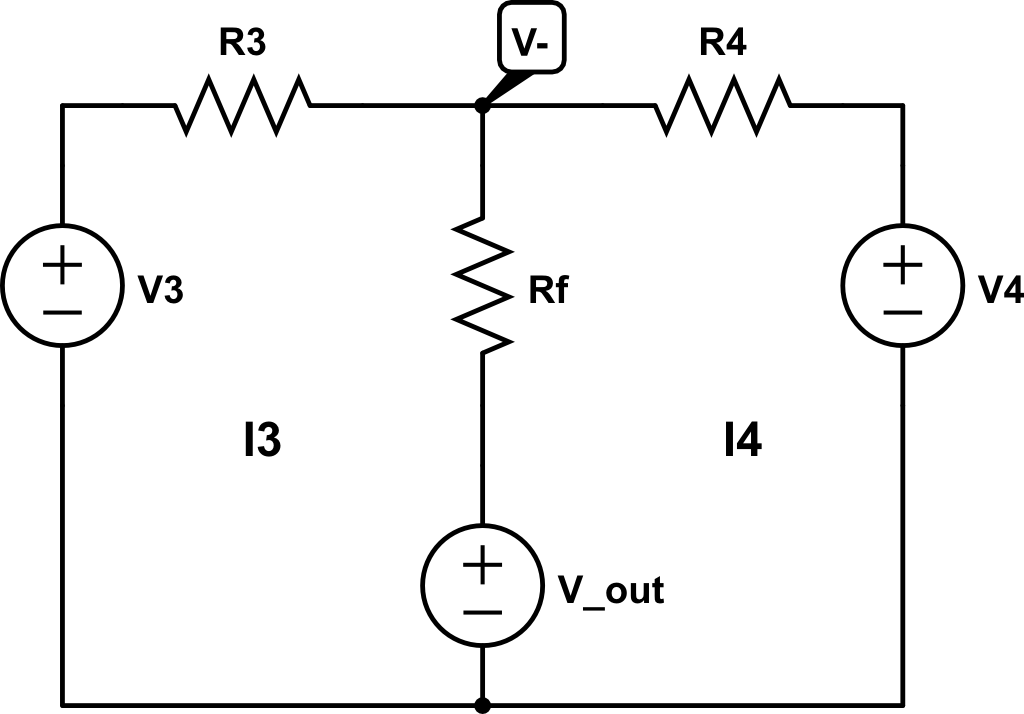
\includegraphics[width=6cm]{lab1_q2_kvl2.png}
\end{center}
\caption{Equivalent circuit at the non-inverting terminal}
\label{q2_b2}
\end{figure}
$$I_3R_3 = V_3 - V^-$$
$$I_4R_4 = V_4 - V^-$$
$$V^- - V_{out} = (I_3 + I_4)R_f $$
$$\text{Substituting from the above equations, we get:}$$
$$ V^- - V_{out} = \Big( \frac{ V_3 - V^-}{R_3} + \frac{ V_4 - V^-}{R_4}\Big) \ R_f$$
$$\text{Reordering the terms, we get:}$$
$$V_{out} =V^- -  \Big( \frac{ V_3 - V^-}{R_3} + \frac{ V_4 - V^-}{R_4}\Big) \ R_f $$
$$\implies V_{out} =V^- \Big( \frac{R_f}{R_3} + \frac{ R_f}{R_4} + 1\Big) - \Big( \frac{R_f}{R_3}\Big)V_3 - \Big( \frac{ R_f}{R_4}\Big)V_4$$

We also know that for an ideal op-amp, $V^+ = V^-$, hence we get:
$$ V_{out} = \Big( \frac{R_f}{R_3} + \frac{ R_f}{R_4} + 1\Big) \Big( \frac{1}{\frac{R_1}{R_g} + \frac{R_1}{R_2} + 1}\Big) V_1 + \Big( \frac{R_f}{R_3} + \frac{ R_f}{R_4} + 1\Big) \Big( \frac{1}{\frac{R_2}{R_g} + \frac{R_2}{R_1} + 1} \Big) V_2 - \Big( \frac{R_f}{R_3}\Big)V_3 - \Big( \frac{ R_f}{R_4}\Big)V_4$$

This is equation is the mathematical representation of the problem statement which which required $V_{out} = a_1V_1 + a_2 V_2 - a_3 V_3 - a_4 V_4$, i.e. :
$$a_1 =  \Big( \frac{R_f}{R_3} + \frac{ R_f}{R_4} + 1\Big) \Big( \frac{1}{\frac{R_1}{R_g} + \frac{R_1}{R_2} + 1}\Big) = 1$$
$$a_2 =  \Big( \frac{R_f}{R_3} + \frac{ R_f}{R_4} + 1\Big) \Big( \frac{1}{\frac{R_2}{R_g} + \frac{R_2}{R_1} + 1} \Big) = 2$$
$$a_3 = \Big( \frac{R_f}{R_3}\Big) = 3$$
$$a_4 = \Big( \frac{ R_f}{R_4}\Big) = 4$$


\subsection*{c}
While building this circuit, we made the following assumptions:
\begin{itemize}
\item The op-amps we use are ideal, i.e. the input impedance is infinite and the output impedance is negligible. This implies that the op-amp does not load it's input circuit and loading effects are not seen on the op-amps output terminal.

\item The voltage at the inverting terminal is equal to the voltage at the non-inverting terminal.

\item The open loop op-amp gain is infinite.

\item The op-amp will operate in an ideal manner when the output is not saturated above or below its supply limits.

\item We used potentiometers to tune the resistors to their required value but none of the components used were ideal components. But for the most part we assumed the values of the resistors were accurate and that capacitors had negligible internal resistance.

\end{itemize}

\subsection*{d}
We started by choosing $R_f$, $R_g$ and $R_g$ to arbitrary resistances such that they were large enough to make sure that other resistances in the circuit were not small. By this we mean that the values of the other resistances were in the order of $k\Omega$. From section \textbf{b}, we can rewrite gains $a_1$ and $a_2$ in terms of $a_3$ and $a_4$ as follows:
$$a_1 =  \Big( a_3 + a_4 + 1\Big) \Big( \frac{1}{\frac{R_1}{R_g} + \frac{R_1}{R_2} + 1}\Big) = 1$$
$$ =  (8) \Big( \frac{1}{\frac{R_1}{R_g} + \frac{R_1}{R_2} + 1}\Big) = 1$$
We can rewrite this  as:
$$8R_2R_g = R_1R_2 + R_1R_g $$
$$\implies R_g = \frac{R_1R_2}{7R_2 - R_1}$$
Similarly for $a_2$, we see:
$$a_2 =  \Big(  a_3 + a_4  + 1\Big) \Big( \frac{1}{\frac{R_2}{R_g} + \frac{R_2}{R_1} + 1} \Big) = 2$$
$$ =  ( 8) \Big( \frac{1}{\frac{R_2}{R_g} + \frac{R_2}{R_1} + 1} \Big) = 2$$
We can re-arrange and re-write the above equations as:
$$R_g = \frac{R_1R_2}{3R_1 - R_2}$$
Equating the two equations which equal $R_g$, we get:
$$ \frac{R_1R_2}{7R_2 - R_1} = \frac{R_1R_2}{3R_1 - R_2}$$
Thus, we get:
$$R_2 = \frac{R_1}{2}$$
Thus we arbitrarily chose $R_f = R_g = 10 \ K\Omega$ and $R_1 = 50 \ K\Omega$
The list of components we ended up using in our circuit can be seen in table 4\ref{q2_tabD}.
\begin{table}[h]
\begin{center}
    \begin{tabular}{|c|c|c|}
        \hline
        \textbf{Component Name} & \textbf{Component Type} & \textbf{Component Specification} \\ \hline
	$ LM 741$                     & \text{Signal Op-amp}         & $ \ V+ = +15V, V- = -15V     $             \\	
       	$ R_f  $                  & \text{Resistor}         & $9.880 \ K\Omega            $        \\ 
	$ R_g $                    & \text{Resistor}         & $9.860 \ K\Omega        $            \\ 
       $ R_1$                     & \text{Resistor}         & $49.3 \ K\Omega        $             \\ 
       $ R_2 $                   & \text{Resistor}         & $24.65 \ K\Omega     $               \\ 
       $ R_3 $                   & \text{Resistor}         & $3.293 \ K\Omega   $                 \\ 
       $ R_4$                     & \text{Resistor}         &$ 2.470 \ K\Omega$                    \\
        \hline
    \end{tabular}
\end{center}
\label{q2_tabD}
\caption{Capacitances and Resistances to construct the summation circuit}
\end{table}

While choosing the components we ensured that the wattage rating of the components were at least equal to or exceeded the power supply of the circuit. As little or no current passes through the circuit\footnote{The system doesn't draw much power and the output of the system is connected to a measuring device which also theoretically draws no current.}, we used $V^2/ R$ to determine the power rating. In every case, the minimum power rating of the component exceeded the circuit power ratings.


\subsection*{e} 
To obtain the resistances specified above we used a combination of potentiometers and fixed resistors which were assembled and then tunned to the correct resistance using a multi-meter. 

\subsection*{f} 
After constructing the circuit as detailed above we began by feeding the following DC signals into our system and measuring the output to confirm its functionality.  These results can be seen in table \ref{q2_ft1}.

\begin{table}[hbt]
\begin{center}
    \begin{tabular}{|c|c|c|c|c|c|c|}
        \hline
        Set & V1 (VDC) & V2 (VDC) & V3 (VDC) & V4 (VDC) & Expected Vout (VDC) & Actual Vout (Avg V) \\ \hline
        1 & 2        & 4        & 1        & 3        & -5                  & -4.9177             \\ 
        2 & 6        & 4        & 2        & 1        & 4                   & 4.0988              \\ 
        3 & 6        & 7        & 2        & 3        & 2                   & 2.17                \\
        \hline
    \end{tabular}
\end{center}
\caption{DC inputs, Expected Output, and Actual Output}
\label{q2_ft1}
\end{table}

The actual voltages in table \ref{q2_ft1} were obtained by averaging the output voltage for several seconds in matlab.
The inputs and outputs for Set 3 are shown in figure \ref{q2_f1}.

\begin{figure}[h]
\begin{center}
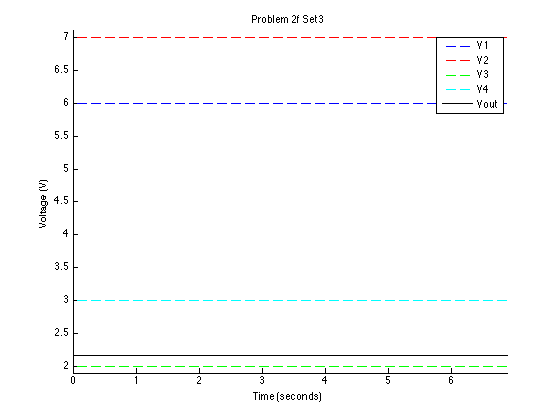
\includegraphics[width=10cm]{problem2f_set3.png}
\end{center}
\caption{Set 3 Inputs and Outputs};
\label{q2_f1}
\end{figure}

Our VI for generating these inputs and reading the outputs is shown in figure \ref{q2_f2}

\begin{figure}[h]
\begin{center}
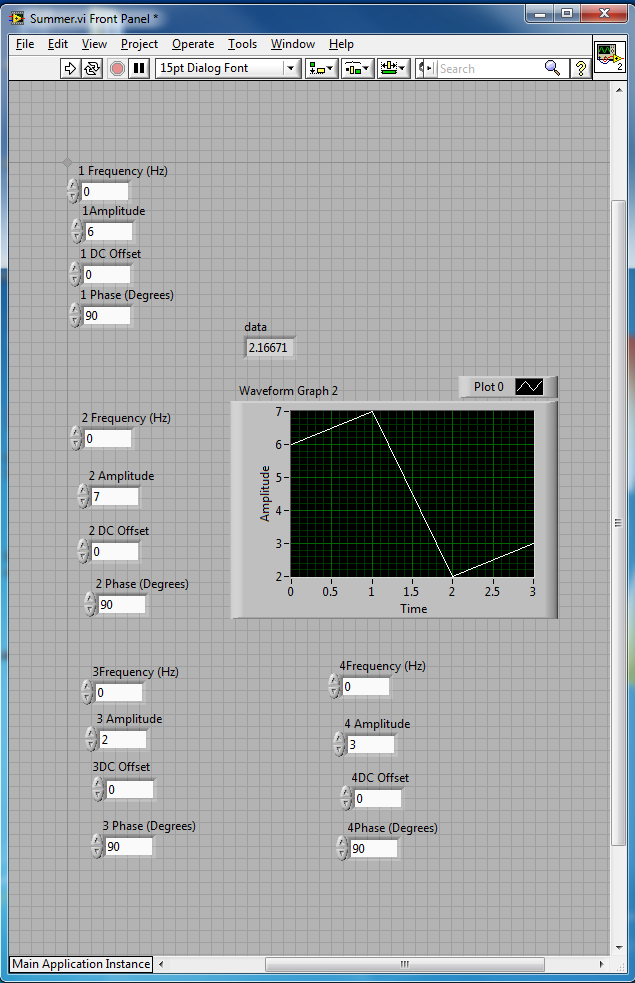
\includegraphics[width = 10cm]{set3problem2.png}
\end{center}
\caption{Set 3 VI};
\label{q2_f2}
\end{figure}

\subsection*{g}
After confirming that the circuit functioned correctly on DC signals we moved on to feed in AC signals and record the output.  These inputs are shown in table \ref{q2_gt1}.  Figure \ref{q2_gf1} shows the output for set 1 superimposed on the simulated inputs and the expected output of the system.  Figure \ref{q2_gf2} shows the output for set 2 superimposed on the simulated inputs to the system and the expected output of the system, while figure \ref{q2_gf3} shows this output within LabView for confirmation.

\begin{table}
\begin{center}
    \begin{tabular}{|c|c|c|c|c|c|c|c|c|}
        \hline
        Set       & Set 1 & ~  & ~  & ~  & Set 2 & ~  & ~  & ~  \\ \hline
        Inputs    & V1    & V2 & V3 & V4 & V1    & V2 & V3 & V4 \\ 
        Amplitude (V) & 3     & 6  & 0  & 0  & 0     & 0  & 2  & 3  \\ 
        Frequency (Hz) & 4     & 4  & 0  & 0  & 0     & 0  & 2  & 2  \\ 
        Offset    (V) & 0     & 0  & 0  & 0  & 0     & 0  & 2  & 0  \\ 
        Phase     (Degrees) & 0     & 90 & 0  & 0  & 0     & 0  & 0  & 45 \\
        \hline
    \end{tabular}
\end{center}
\caption{Set 1 and Set 2 inputs}
\label{q2_gt1}
\end{table}



\begin{figure}[hbt]
\begin{center}
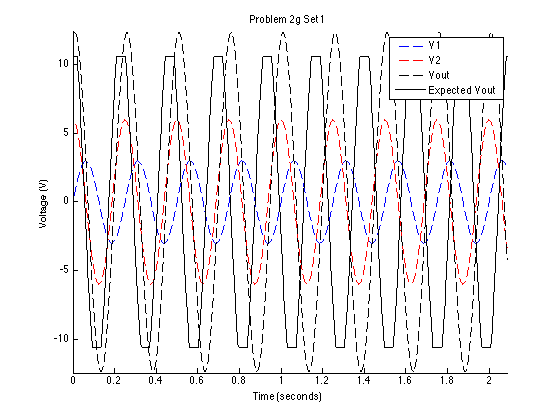
\includegraphics[width = 15cm]{problem2g_set1.png}
\caption{Set 1 Input and Output}
\label{q2_gf1}
\end{center}
\end{figure}

\begin{figure}[hbt]
\begin{center}
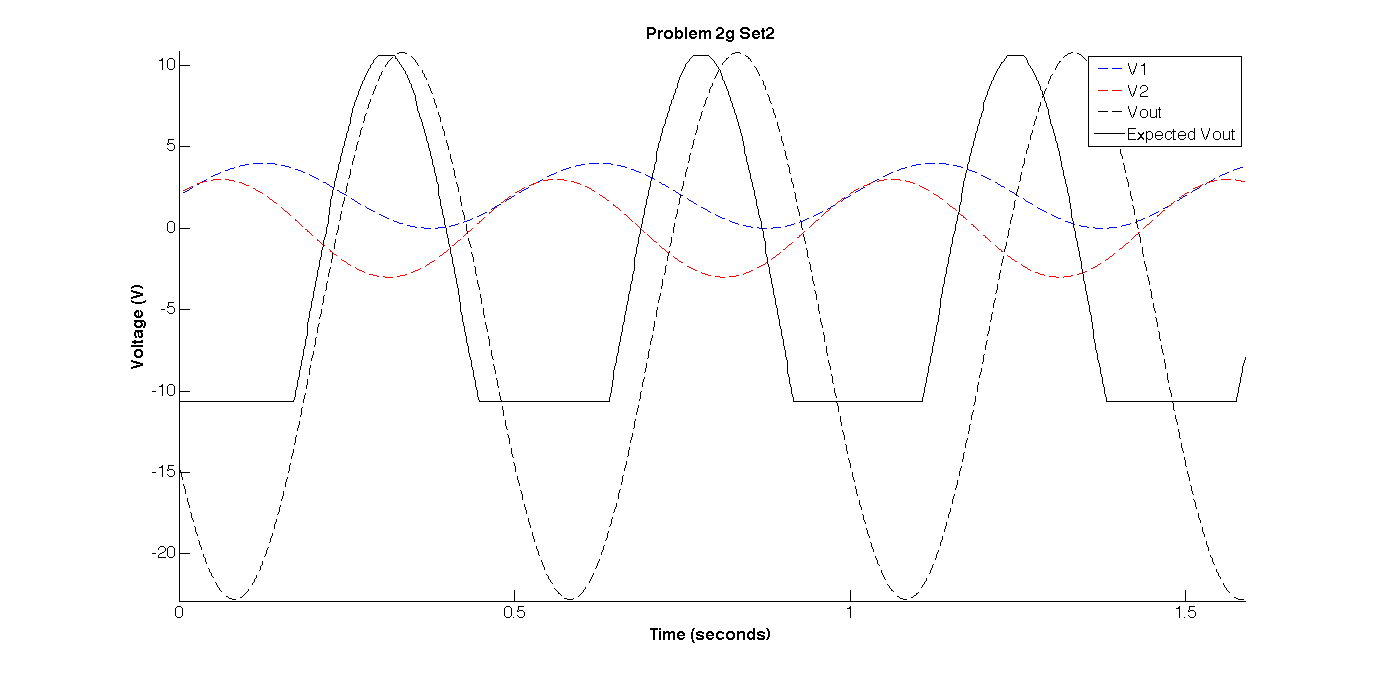
\includegraphics[width = 15cm]{problem2g_set2.png}
\caption{Set 2 Input and Output}
\label{q2_gf2}
\end{center}
\end{figure}

\begin{figure}[hbt]
\begin{center}
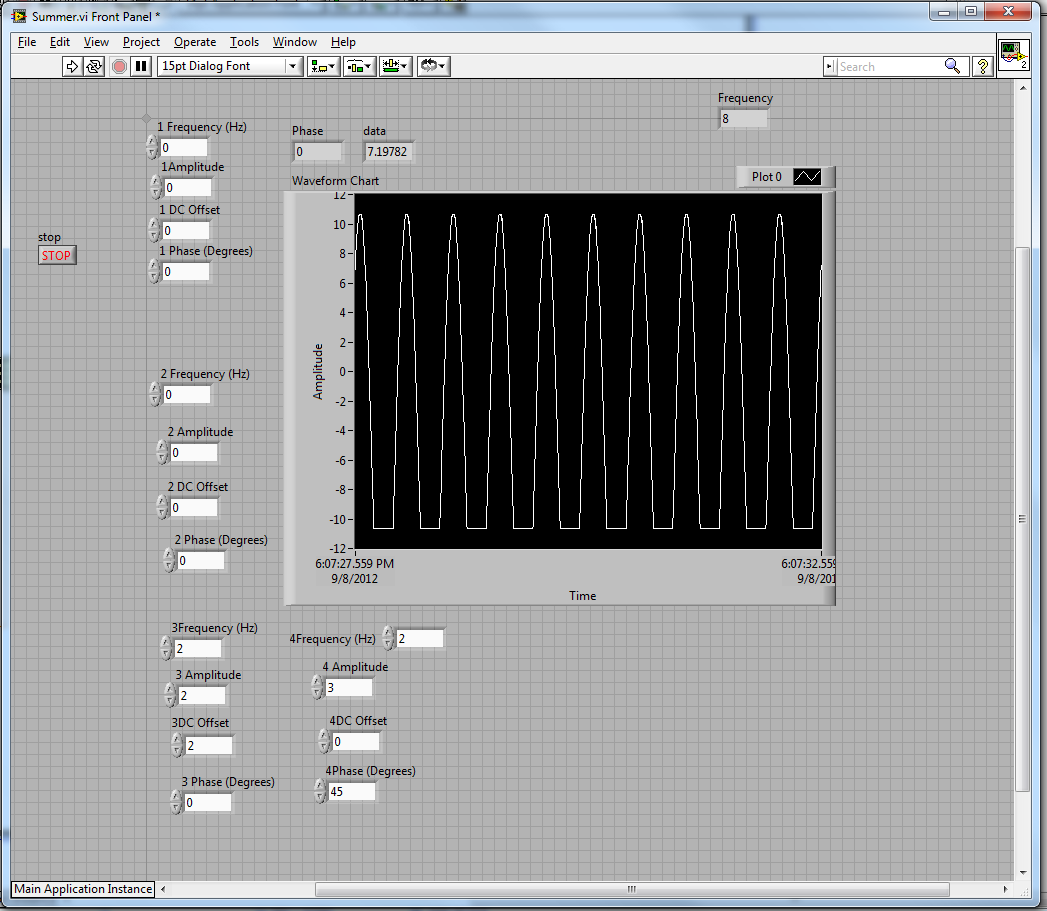
\includegraphics[width = 10cm]{set2partgproblem2.png}
\caption{Set 2 Output within LabView}
\label{q2_gf3}
\end{center}
\end{figure}

Both figure \ref{q2_gf1} and figure \ref{q2_gf2} show a close correspondence between the actual and expected output with a few notable differences.  The most  obvious difference is the lag between the actual output and the expected output.  When generating these graphs we assume a uniform 1 ms sampling period, which turns out to not be the case when examining real timing data.  This discrepancy is the result of the system requesting a sample, since we are using on demand sampling, but not receiving the sample in time.  As a consequence of this the time difference between some of the output samples are larger than 1 ms, which on a whole cause fewer than 1000 samples to be taken per second.  This compresses the graph along the time axis resulting in a graph that is out of sync with the expected results.  This issue could be easily remedied by storing the sampled amplitude and the sample time and plotting the amplitude against the actual time rather than the theoretical time.  \\

Both figure \ref{q2_gf1} and figure \ref{q2_gf2} also illustrate a saturation effect at $\pm$ 11 volts.  For an ideal op-amp we would expect the output to saturate at the supply voltages which were confirmed to be  $\pm$ 15 volts. However we would not expect a real op-amp, such as our LM741, to output voltages all the way up to the supply voltage, but rather within about 2 volts of the supply.  But this does not explain the saturation at $\pm$ 11 volts.  Examining the data sheet of our DAQ, the NI 6230 reveals a maximum input voltage of $\pm$ 10 volts.  It is likely that the designers are being somewhat conservative in their estimate of input ranges, so a saturation at 11 volts is likely due to the limited range of the DAQ.


\subsection*{h} 
The beating signal is achieved as a sinusoidal wave which has an amplitude that also varies sinusoidally. In effect, the output is $\sin(\omega_a t)\sin(\omega_b t) $. We can use trigonometric identities to rearrange this sinusoidal product as a sum as follows:
$$\sin(\omega_a t)\sin(\omega_b t) = \frac{\cos(\omega_a t + \omega_b t) - \cos(\omega_a t + \omega_b t)}{2}$$
We use the product-to-sum identity to break up the product of the sines into a sum of cosines. We can again rewrite the cosines in terms of sines by taking into account the phase difference.
$$\frac{\cos(\omega_a t + \omega_b t) - \cos(\omega_a t + \omega_b t)}{2} = \frac{\sin((\omega_a t + \omega_b t) + \pi/2)- \sin((\omega_a t + \omega_b t) + \pi/2)}{2}$$

This way, we can achieve a beating signal as a sum of sinusoids. For the purposes of this question, we chose $\omega_a = 1$ and $\omega_b = 10$ The values for each of the output terminals is as follows:
\begin{table}[hbt]
\begin{center}
    \begin{tabular}{|c||c|c|c|c|}
        \hline
        ~                 & V1              & V2 & V3              & V4 \\ \hline \hline
        Amplitude (Volts) & 3               & 0  & 1               & 0  \\ \hline
        Frequency (Hz)    & -9              & 0  & 11              & 0  \\ \hline
        Offset (Volts)    & 0               & 0  & 0               & 0  \\ \hline
        Phase (Radians)            & $\frac{\pi}{2}$ & 0  & $\frac{\pi}{2}$ & 0  \\
        \hline
    \end{tabular}
\end{center}
\end{table}

The required LabView screen shot can be seen in figure \ref{q2_h1} while the graph itself may be seen in figure \ref{q2_h2}.

\begin{figure}[hbt]
\begin{center}
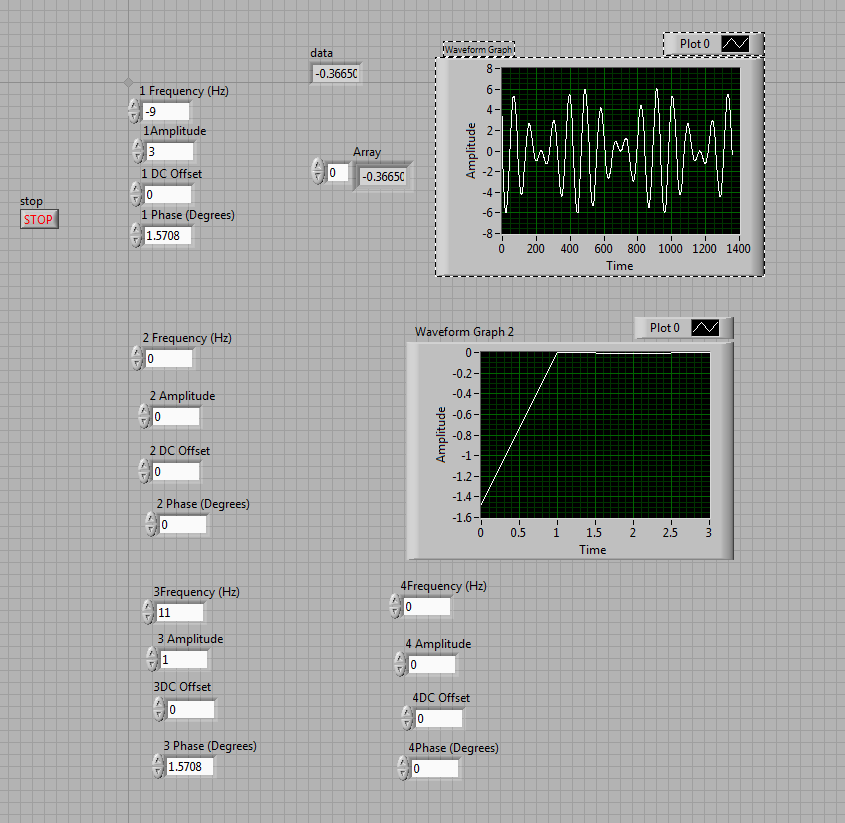
\includegraphics[width=15cm]{problem2_h.png}
\end{center}
\caption{The LabView front-end of a system that produces $\sin(\omega_a t_a)\sin(\omega_b t_b) $.}
\label{q2_h1}
\end{figure}

\begin{figure}[hbt]
\begin{center}
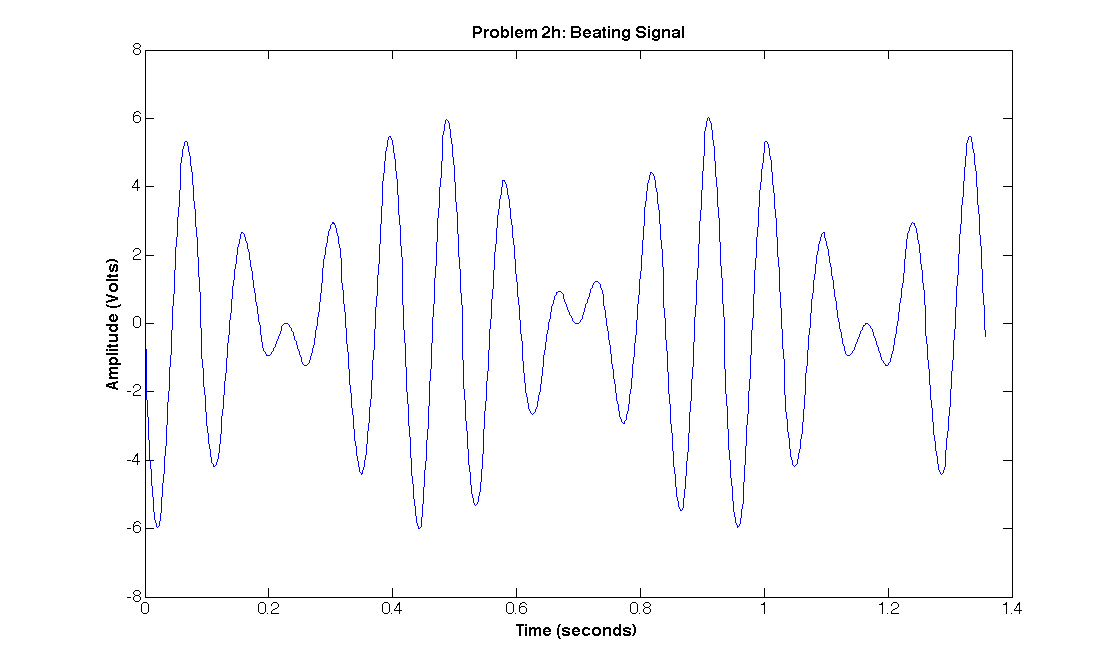
\includegraphics[width = 15cm]{problem2h_plot.png}
\end{center}
\caption{Problem 2h received signal}
\label{q2_h2}
\end{figure}

\newpage
\section*{Teamwork Participation Pledge}

\textbf{Lab 1 : Electronic Circuits}

\vspace{2 cm}

I attest that I have made a fair and equitable contribution to this lab and submitted 
assignment. \\

My signature also indicates that I have followed the University of Michigan Honor Code, 
while working on this lab and assignment.\\

I accept my responsibility to look after all of the equipment assigned to me and my team, 
and that I have read and understood the X50 Lab Rules.\\

\begin{table}[h]
\begin{center}
    \begin{tabular}{|c|c|c|}
        \hline
        \textbf{Name} & \textbf{Email}     & \textbf{ \ \ \ \ \  \ \  \ \ \ \ \  \ \ Signature  \ \ \ \ \  \ \ \ \ \ \ \  \ \ } \\ \hline
        	~& ~& ~\\
	~& ~& ~\\
	Shiva Ghose   & gshiva@umich.edu   & ~                  \\
	~& ~& ~\\
	~& ~& ~\\ \hline 
	~& ~& ~\\
	~& ~& ~\\
        John Peterson & jrpeters@umich.edu & ~                  \\ 
	~& ~& ~\\
	~& ~& ~\\ \hline 
	~& ~& ~\\
	~& ~& ~\\
        Wenjian Bai   & baiwenji@umich.edu & ~                  \\
	~& ~& ~\\
	~& ~& ~\\ \hline 
        \hline
    \end{tabular}
\end{center}
\end{table}



\end{document}





\def\therefore{\boldsymbol{\text{ }
\leavevmode
\lower0.4ex\hbox{$\cdot$}
\kern-.5em\raise0.7ex\hbox{$\cdot$}
\kern-0.55em\lower0.4ex\hbox{$\cdot$}
\thinspace\text{ }}}
